\documentclass[a4paper,11pt]{amsart}
\usepackage{amssymb}
\usepackage{graphicx}

\parskip 1ex
\parindent 0 pt

\newcounter{temp}
\newcounter{prob_counter}
\newcounter{sprob_counter}

\newenvironment{problem}
{\begin{list}{{\bf \arabic{prob_counter}}}{
      \usecounter{prob_counter}
      \addtolength{\labelsep}{.6ex}
      \addtolength{\itemsep}{4.3ex}
      \setlength{\leftmargin}{1.4em}}
      \setcounter{prob_counter}{\value{temp}}
}
{\setcounter{temp}{\value{prob_counter}}  
  \end{list}
}

\newenvironment{subprob}
{
  \begin{list}{{\bf \alph{sprob_counter}}}{
      \usecounter{sprob_counter}
      \addtolength{\labelsep}{.6ex}
      \addtolength{\itemsep}{.5ex}
      \setlength{\leftmargin}{1.7em}}
}
{\end{list}}

\newenvironment{solution}{\textbf{Solution.}}{\qed}

\newcommand{\rubrik}[1]{\bigskip \begin{center}{\bf #1}\end{center} \medskip}

\newcommand{\NN}{\mathbb{N}}
\newcommand{\ZZ}{\mathbb{Z}}
\newcommand{\QQ}{\mathbb{Q}}
\newcommand{\RR}{\mathbb{R}}




\begin{document}

\pagestyle{empty}
\thispagestyle{empty}

{\small{\sc\noindent
        Sebastian Plenz ({\tt sebastianp16@ru.is}) and Tigran Tonoyan ({\tt tigran@ru.is})
}}

\rubrik{PROBLEM SET 6 (T-445-GRTH)}

You need to collect $\bf 65$ points to get a full score {\bf but} you cannot get more than {\bf X} points (in total) from a problem section with annotation {\bf max X}.

{\bf Please make sure to:}\\
1. Write your name/email(s) on your work (replace my name above).\\
2. Write your answers in \texttt{{\textbackslash}begin\{solution\} ... {\textbackslash}end\{solution\}} blocks.\\
3. Write clear and concise proofs: points may be deducted for vagueness.




\section{Intersection, Chordal, Outerplanar Graphs ({\bf max 55})}

{\bf Definition.} A planar graph $G$ is \emph{outerplanar} if $G$ has an embedding in the plane in such a way that every vertex is on the boundary of the infinite face.

\begin{problem}
 \item (5 points) Prove that every connected unit interval graph has a Hamiltonian path.
\end{problem}
\begin{solution}
	Take a unit interval representation of the graph and order the intervals from the lowest beginning to the highest one. Begin the path at the vertex of the first interval and connect it to the second one and so one. This is possible because it is a connected graph and the intervals all have the same length, so there exists no interval, that is a proper subset of an other interval.
\end{solution}

\begin{problem}
\item (8 points) Prove that every outerplanar graph on $n$ vertices has at most $2n-3$ edges.
\end{problem}
\begin{solution}
	We prove the claim by induction. For n=1,2 or 3, it is trivial. \\
	The assumption holds for an aribtrary n. \\
	Take an outerplanar graph on n+1 vertices. We delete a vertex with degree less or equal to 2. The remaining graph is still an outerplanar graph and has at most $2n-3$ edges by induction hypothesis. So the graph on $n+1$ vertices has at most $2(n+1)-3$ wich shows the assumption. \\
	It reamains to show, that there exists a vertex of degree less or equal to two. Either you have a leaf. Than it is true. If not, the outer edges form a cycle. If there are no inner edges, it is true. If there is an inner edge, it can not connect two adjacent vertices. There need to be one in between, with degree 2. So the assumption holds.
\end{solution}

\begin{problem}
\item (10 points) Let $G$ be a graph in which any two simple cycles have at most one vertex in common. 
\begin{subprob}
\item Let $B$ be a block in $G$. What can you say about the structure of $B$?
\item Prove that $G$ is an outerplanar graph.
\end{subprob}
\end{problem}
\begin{solution}
	a) B is at most 2-connected. \\
	b) 
\end{solution}

\begin{problem}
\item (7 points) Prove that every unit coin graph on $n > 3$ vertices has at most $3n-7$ edges.
\end{problem}
\begin{solution}
	A vertex can have at most 6 neighbors by geometrical properties. We take a representation with unic coins and order it from left to right. Take the leftmost vertex. It only has neigbors to his right and therefor maximal three. By inductuion, the claim holds if it is true for a base case. Take 4 vertices. They can maximal have 5 edges. So the assumption holds. 
\end{solution}


\begin{problem}
\item (8 points) Prove that for any unit disc graph $G$, $D(G) \le 3(\omega(G)-1)$.
\end{problem}



\begin{problem}
 \item (20 points) A graph $G$ is a {\em split graph} if $V(G)$ can be partitioned into subsets $X,Y$, such that $G[X]$ is a clique and $G[Y]$ is a null graph.
 \begin{subprob}
  \item Prove that split graphs are chordal.
  \item Prove that the complement of a split graph is a split graph.
  %\item Let $G = (X, Y, E)$ be a split graph. Is it true that if $G$ is self-complementary (meaning $G$ is isomorphic to $\overline{G}$), then $|X|=|Y|$?
  \item Find a split graph that is not an interval graph.
 \end{subprob}
\end{problem}
\begin{solution}
	a) Let $G'$ be any induced subgraph. If it contains only vertices from the clique, it is obviously triangulated. If it does not contain only vertices from the clique, it is not an induced cycle, because one vertex is isolated. \\
	b) The complement of a complete graph is a null graph and the other way around. So our partition is the same as for the original graph. \\
	c) An example is displayed in the following graphic \\
	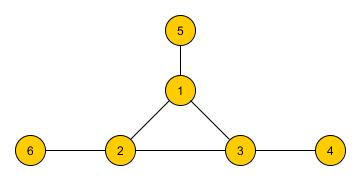
\includegraphics{A6.jpg} \\
	It is not an interval graph, because the vertices 1,2 and 3 need to have something in common, but each of them needs to have an end, that is not the same as the others. This is only possible for two of them. 
\end{solution}

\begin{problem}
 \item (20 points) A graph $G$ is a \emph{threshold graph} if there is a non-negative number $B$ and a non-negative number $a_v$ for each vertex $v\in V(G)$, such that for any subset $U \subseteq V(G)$, $U$ is an independent set \emph{if and only if} $\sum_{v\in U} a_v \le B$.
Use this definition of threshold graphs to prove:
\begin{subprob}
 \item $K_n$ is a threshold graph.
 \item Adding an isolated vertex to a threshold graph gives a threshold graph.
 \item Adding a dominating vertex (a vertex that is connected to 
 every other vertex) to a threshold graph gives a threshold graph. 
 \item Every threshold graph is a split graph.
\end{subprob}
Note: \emph{Every} threshold graph can be built by repeatedly doing the two operations above (no proof required).
\end{problem}



\section{Powers of Graphs}


\begin{problem}
\item (5 points) Let $\{[a_1, b_1], \ldots, [a_n, b_n]\}$ be an interval representation of a graph $G$.
Show that $\{[a_1, b'_1], \ldots, [a_n, b'_n]\}$, where $$b'_i = \max_j \{b_j : \mbox{$[a_j, b_j]\cap [a_i, b_i] \neq \emptyset$} \},$$ is an interval representation of the graph $G^2$.
\end{problem}


\begin{problem}
\item (10 points) Let $T$ be a tree. Show that $\chi(T^2) = \Delta(T) + 1$.
\end{problem}



\section{Perfect Graphs}


\begin{problem}
 \item (8 points) Prove that the complement of an odd cycle $C_{2k+1}$ with $k>1$ is  not a perfect graph.
\end{problem}
\begin{solution}
	The complement of $C_5$ is again $C_5$. $C_5$ is not perfect, because the chromatic number is 3 but the clique number is 2. Take an odd cycle as in the task. Number the edges once around in a circle. Take the complement a graph. It has a subgraph, that is a 5cycle. For example, We can take the cycle along the vertices 1,3,5,2,4,1. 
\end{solution}

\begin{problem}
 \item (10 points) Let $G,H$ be two perfect graphs whose intersection is a complete graph. Prove that $G \cup H$ is perfect.
\end{problem}
\begin{solution}
	Take an arbitray subset $S$ of vertices of $G \cup H$. If it contains only vertices from one of these graphs, it is perfect. Assume, that it contains vertices from both graphs. Wlog the subset is connected (unconnected things don't change the chromatic or the clique numbers). Take the two subsets $S_1=S \cap G$ and $S_2=S \cap H$. For both subsets, the chromatic and the clique number are the same. Because the vertices in common form a complete graph, they all have different colors. So the we take the higher cliqu number and the higher chromatic number. This are the numbers of our subset, so the graph is perfect.
\end{solution}

\begin{problem}
\item (9 points) Show that perfection is closed neither under edge deletion nor (simple) contractions.
\end{problem}
\begin{solution}
	Take $C_6$. It is perfect but contraction by any edge results in $C_5$, that is not perfect. \\
	Take $C_5$ and connect two adjacent vertices to a new vertex. This graph is perfect, but deleting one of the two edges, that are not in $C_5$ result in a not perfect graph. 
\end{solution}




\section{Claw-Free Graphs}

{\bf Definition.} A \emph{claw} graph is a star with three leaves, i.e. has four vertices, three of them adjacent to the fourth one. A graph is \emph{claw-free} if it doesn't contain a claw as an \emph{induced} subgraph. 

{\bf Definition.} The line graph $L(G)$ of a graph $G$ is such that each vertex of $L(G)$ represents an edge of $G$, and two vertices of $L(G)$ are adjacent if and only if their corresponding edges are incident in $G$ (share a vertex). For instance, the line graph of a star is a complete graph.

\begin{problem}
 \item (5 points) Prove that the complement of a triangle-free graph is claw-free.
\end{problem}

\begin{problem}
 \item (5 points) Prove that for any graph $G$, the line graph $L(G)$ is claw-free. 
\end{problem}

\begin{problem}
 \item (7 points) Prove that for any claw-free graph $G$, $\frac{\Delta(G)}{2} \le \chi(G)\le \Delta(G)+1$. 
\end{problem}

\begin{problem}
 \item (6 points) Prove that every claw-free interval graph is a unit interval graph (i.e. the class of claw-free interval graphs is precisely the class of unit interval graphs).
\end{problem}






\end{document}

